%%%%%%%%%%%%%%%%%%%%%%%%%%%%%%%%%%%%%%%%%
% "ModernCV" CV and Cover Letter
% LaTeX Template
% Version 1.2 (25/3/16)
%
% This template has been downloaded from:
% http://www.LaTeXTemplates.com
%
% Original author:
% Xavier Danaux (xdanaux@gmail.com) with modifications by:
% Vel (vel@latextemplates.com)
%
% License:
% CC BY-NC-SA 3.0 (http://creativecommons.org/licenses/by-nc-sa/3.0/)
%
% Important note:
% This template requires the moderncv.cls and .sty files to be in the same 
% directory as this .tex file. These files provide the resume style and themes 
% used for structuring the document.
%
%%%%%%%%%%%%%%%%%%%%%%%%%%%%%%%%%%%%%%%%%

%----------------------------------------------------------------------------------------
%	PACKAGES AND OTHER DOCUMENT CONFIGURATIONS
%----------------------------------------------------------------------------------------

\documentclass[11pt,a4paper,sans]{moderncv} % Font sizes: 10, 11, or 12; paper sizes: a4paper, letterpaper, a5paper, legalpaper, executivepaper or landscape; font families: sans or roman
\usepackage[utf8]{inputenc}

\moderncvstyle{casual} % CV theme - options include: 'casual' (default), 'classic', 'oldstyle' and 'banking'
\moderncvcolor{blue} % CV color - options include: 'blue' (default), 'orange', 'green', 'red', 'purple', 'grey' and 'black'

\usepackage{lipsum} % Used for inserting dummy 'Lorem ipsum' text into the template

\usepackage[scale=0.75]{geometry} % Reduce document margins
%\setlength{\hintscolumnwidth}{3cm} % Uncomment to change the width of the dates column
%\setlength{\makecvtitlenamewidth}{10cm} % For the 'classic' style, uncomment to adjust the width of the space allocated to your name

%----------------------------------------------------------------------------------------
%	NAME AND CONTACT INFORMATION SECTION
%----------------------------------------------------------------------------------------

\firstname{Imanol} % Your first name
\familyname{Studer} % Your last name

% All information in this block is optional, comment out any lines you don't need
\title{Curriculum Vitae}
\address{Wickenweg 51}{8048 Zürich}
\mobile{+41 (0)76 462 67 16}
% \phone{}
% \fax{}
\email{imanol.studer@gmail.com}
% \homepage{}{} % The first argument is the url for the clickable link, the second argument is the url displayed in the template - this allows special characters to be displayed such as the tilde in this example
% \extrainfo{}
\photo[70pt][0.4pt]{pictures/picture} % The first bracket is the picture height, the second is the thickness of the frame around the picture (0pt for no frame)
% \quote{}

%----------------------------------------------------------------------------------------

\begin{document}

%----------------------------------------------------------------------------------------
%	COVER LETTER
%----------------------------------------------------------------------------------------

% To remove the cover letter, comment out this entire block

%\clearpage
%
%\recipient{HR Department}{Corporation\\123 Pleasant Lane\\12345 City, State} % Letter recipient
%\date{\today} % Letter date
%\opening{Dear Sir or Madam,} % Opening greeting
%\closing{Sincerely yours,} % Closing phrase
%\enclosure[Attached]{curriculum vit\ae{}, Master Grades, Bachelor's Diploma} % List of enclosed documents
%
%\makelettertitle % Print letter title
%
%\lipsum[1-3] % Dummy text
%
%\makeletterclosing % Print letter signature
%
%\newpage

%----------------------------------------------------------------------------------------
%	CURRICULUM VITAE
%----------------------------------------------------------------------------------------

\makecvtitle % Print the CV title

%----------------------------------------------------------------------------------------
%	EDUCATION SECTION
%----------------------------------------------------------------------------------------

\section{Education}

\cventry{2014--2016}{Master of Science - Multimodal and Cognitive Systems}{University of Zürich}{}{}{Modules included:
\begin{itemize}
	\item Fundamentals of Image Processing and Computer Vision
	\item Autonomous Mobile Robots
	\item Introduction to Machine Learning (ETH Course)
	\item Neuromorphic Engineering II
	\item Neurophysics
	\item Complex Systems: Berechenbares Chaos in dynamischen Systemen
	\item Master Project: Head Pose Tracking with Quadrotors
\end{itemize}}  % Arguments not required can be left empty

\cventry{2009--2013}{Bachelor of Science - Applied Informatics: Neuroinformatics}{University of Zürich}{}{}{Modules included:
\begin{itemize}
	\item Neuromorphic Engineering I
	\item Theory, Programming and Simulation of Neural Networks
	\item Systems Neuroscience
	\item Computational Vision
	\item Introduction to Neuroinformatics
\end{itemize}}

\cventry{2008--2009}{Passerelle}{AKAD College}{}{}{The Passerelle is an exam which, together with a Berufsmatura, qualifies as a Matura and allows studying at a University.}

\cventry{2003--2007}{Informatikmittelschule}{Kantonsschule Enge}{}{}{
The Informatikmittelschule provides a practically oriented education as a programmer and is similar to an apprenticeship. The first three years consist of programming lessions and standard school subjects with a focus on economics. Finally, there are exams and a Berufsmatura is obtained. The last year is an internship, including a two week project, which must be done at a company. My project was a prototype of a chemical monitoring system for water recycling plants.}

\cventry{1999--2003}{Gymnasium, Ancient language profile}{Kantonsschule Freudenberg}{}{}{I completed 4 years at the Gymnasium with focus on languages (German, French, Spanish, Latin). After the 4th year I decided to drop it in favour of the Informatikmittelschule because I had lost the interest in languages.}

\section{Masters Thesis}

\cvitem{Title}{\emph{Paper Tracking} - A real time algorithm}
\cvitem{Supervisor}{Prof. Dr. Chat Wacharamanotham}
\cvitem{Description}{I developed an algorithm that is capable of tracking a printed scholarly paper while a person is reading it. The images come from a head mounted camera and are then processed by a laptop. The algorithm scans for high densities of color intensity changes to find the paper. The paper is then clipped from the image and mached against a database of paper PDFs using SURF features. In a final step it scans the PDF in the database for statistical plots by analyzing the figures using visual words based feature vectors and an SVM with an RBF kernel.}
\cvitem{Grade}{\textbf{5.75}}

\section{Bachelor Thesis}

\cvitem{Title}{\emph{Maggie} - An Infant Robot Model}
\cvitem{Supervisor}{Dr. Hugo Gravato Marques}
\cvitem{Description}{I built a physical prototype of an infant robot model including an API to control it from a PC and collect data. It is made out of metal parts, servo motors, force resisting sensors, two cameras, IMUs and 3D designed and printed parts.}
\cvitem{Grade}{\textbf{5.5}}

%----------------------------------------------------------------------------------------
%	WORK EXPERIENCE SECTION
%----------------------------------------------------------------------------------------

\section{Experience}

\cventry{2016--now}{Software Developer}{\textsc{Supercomputing Systems AG}}{Zürich}{}{SCS AG is a former ETH spinoff based in Technopark that develops outsourced software projects for other companies with a focus on embedded systems. So far I have worked in the following projects:
\begin{itemize}
\item RenesasDNN: Renesas is a Japanese car electronics manufacturer that sells its products mainly for german car manufacturers. The RenesasDNN Project is about developing a python utility that allows the user to transform a previosly trained neural network (TensorFlow or Caffe) to be translated so that it runs on a FPGA deep learning accelerator. The FPGA supports fixpoint operation and has a limited tensor size for convolution operations. The python utility thus is responsible for dividing the large matrix multiplications and convolutions into smaller ones and converting the network parameters from float to fixpoint. We applied a ristretto-like approach. I was personally responsible for the implementation of standard network layers such as convolution, multiplication and maxpool and for the fix point quantization. I implemented the performance consuming parts in C++ and created Python bindings for the integration of the rest of the application.
\newline
\textbf{Skills used}: Deep Learning, Python 3.5, NumPY, GIT, PyCharm, Python Bindings C++14.
\item Gridsense: In this project we developed a load balancing algorithm for the electrical grid. The goal was to schedule the power consumption of electrical home appliances such as boilers, car chargers, batteries to minimize grid voltage fluctuations. This was implemented in the form of Gridsense Units (embedded controllers connected to electrical appliances) and a Device Management System. The Gridsense Units have a master for each home, which uses an MDP algorithm to compute the optimal schedule for the devices in the same household. I was in the team in charge of the Gridsense Units and personally responsible for the core software architecture, part of the build system and IoT interfaces.
\newline
\textbf{Skills used}: C++14, Optimal Control, Iotivity Framework, CMake, GIT, Eclipse
\item Smartbox: This project is similar to Gridsense, except that it does the load balancing optimization on a regional scale instead of in a household. The Smartbox is a devices which is connected to the transformer stations throughout a region and is able to predict voltage fluctuations which enables the grid owner to prevent such events.
I was personally responsible for implementing different modules that calculate different features of the grid signal.
\newline
\textbf{Skills used}: C++03, Eclipse, CMake, GIT, Eclipse, Signal Processing
\item Deutsche Bahn Signal Box, Transformation Frontend: The biggest project of SCS AG is the development of a new signal box for Deutsche Bahn. We are developing a replacement for the old hardware from the 1950s based on FPGA hardware. The Project is being developed according to the SIL4 guidlines and is composed of different subprojects. I was involved in the deveopment of a Utility which allows the user to draw the schematics of the old hardware and translates them into FPGA code for a new hardware. The Utility is being developed in Java and I am responsible for the JavaFX frontend.
\newline
\textbf{Skills used}: Java 9, JavaFX, Maven, GIT Eclipse
\end{itemize}}

\cventry{2012--2015}{Software Developer}{\textsc{New Voice AG}}{Zürich}{}{New Voice AG is a company located in Zürich which develops a software called MobiCall which is an Alarm-, Information-, Conference and Callrecording system which is built on top of a PBX system. My responsibility was to develop and maintain a plugin for locating Dect and WiFi devices inside buildings and triggering alarms.
\newline
\textbf{Skills used}: Python (2.7 and 3.1), C++11, git, SKLearn, Machine Learning, Python Bindings, USB Interface Programming, Qooxdoo, Autobahn, Eclipse}

%------------------------------------------------

\cventry{2011--2012}{Software Developer}{\textsc{TrueBPM Solutions AG}}{Zürich}{}{TrueBPM develops a BPM system that is used internally by an assurance company. While I was working there, I was responsible for letter generation. I had to design BIRT reports based on word documents and also do some server backend programming. I left the company after a year, because the project was finished and I wanted to do something more challenging. 
\newline
\textbf{Skills used}: Java, BIRT Templates, GIT, Eclipse}

%------------------------------------------------

\cventry{2006--2011}{Software Developer}{\textsc{IT-GR GmbH}}{Zürich}{}{IT-Gr GmbH is a software developing company. During my time there I worked alone on a monitoring system for water recycling plants for a customer called Unimon GmbH. The software periodically pulls measured data from different sensors embedded in the water plant. Users can log in through a web interface, analyze the data and create reports. It is also possible to define conditions under which alarms are  triggered. It then automatically contacts the responsible person per E-Mail or SMS. I was the only developer involved in the project. 
\newline
My first year there (2006-2007) was an Internship as part of the “Informatikmittelschule”.
\textbf{Skills used}: Java, git, eclipse, JBoss, Seam Framework, MySQL, Linux Server Administration, testing and requirements specification.}

%----------------------------------------------------------------------------------------

%----------------------------------------------------------------------------------------
%	REFERENCE CONTACTS SECTION
%----------------------------------------------------------------------------------------

\newpage

\section{Reference Contacts}

\subsection{Prof. Dr. Chat Wacharamanotham}
\cvitem{Link}{\href{http://www.ifi.uzh.ch/en/zpac/people/chat.html}{http://www.ifi.uzh.ch/en/zpac/people/chat.html}}
\cvitem{}{Supervision of Master Thesis}
\cvitem{E-Mail}{\href{mailto:chat@ifi.uzh.ch}{chat@ifi.uzh.ch}}

\subsection{Prof. Dr. Davide Scaramuzza}
\cvitem{Link}{\href{http://rpg.ifi.uzh.ch/people\_scaramuzza.html}{http://rpg.ifi.uzh.ch/people\_scaramuzza.html}}
\cvitem{}{Supervision of Master Project}
\cvitem{E-Mail}{\href{mailto:sdavide@ifi.uzh.ch}{sdavide@ifi.uzh.ch}}

%----------------------------------------------------------------------------------------
%	COMPUTER SKILLS SECTION
%----------------------------------------------------------------------------------------

\section{Computer skills}

\cvitem{Basic}{\textsc{Bash Scripts}, \textsc{QT}, \textsc{Cuda}, \textsc{Reinforcement Learning}, \textsc{Natural Language Processing}, \textsc{Optimal Control}}
\cvitem{Intermediate}{\textsc{java}, \textsc{html}, \textsc{JavaScript}, \LaTeX, \textsc{Microsoft Windows}, \textsc{OpenCV}, \textsc{Computer Hardware}, \textsc{Scikit Learn}}
\cvitem{Advanced}{\textsc{python}, \textsc{C++}, \textsc{Linux}, \textsc{Deep Learning}, \textsc{Machine Learning}}

%----------------------------------------------------------------------------------------
%	LANGUAGES SECTION
%----------------------------------------------------------------------------------------

\section{Languages}

\cvitemwithcomment{German}{Mothertongue}{}
\cvitemwithcomment{Spanish}{Mothertongue}{}
\cvitemwithcomment{English}{Proficient}{}

%----------------------------------------------------------------------------------------

%----------------------------------------------------------------------------------------
%	INTERESTS SECTION
%----------------------------------------------------------------------------------------

\section{Interests}

\renewcommand{\listitemsymbol}{-~} % Changes the symbol used for lists


\cvlistdoubleitem{Reinforcement Learning}{Deep Learning}
\cvlistdoubleitem{Natural Language Processing}{Philosophy}
\cvlistdoubleitem{Reading}{Jiu Jitsu}
\cvlistdoubleitem{Karate}{Cooking}

\newgeometry{bottom=0pt}
\section{Master Grades - Exempt from module booking system}
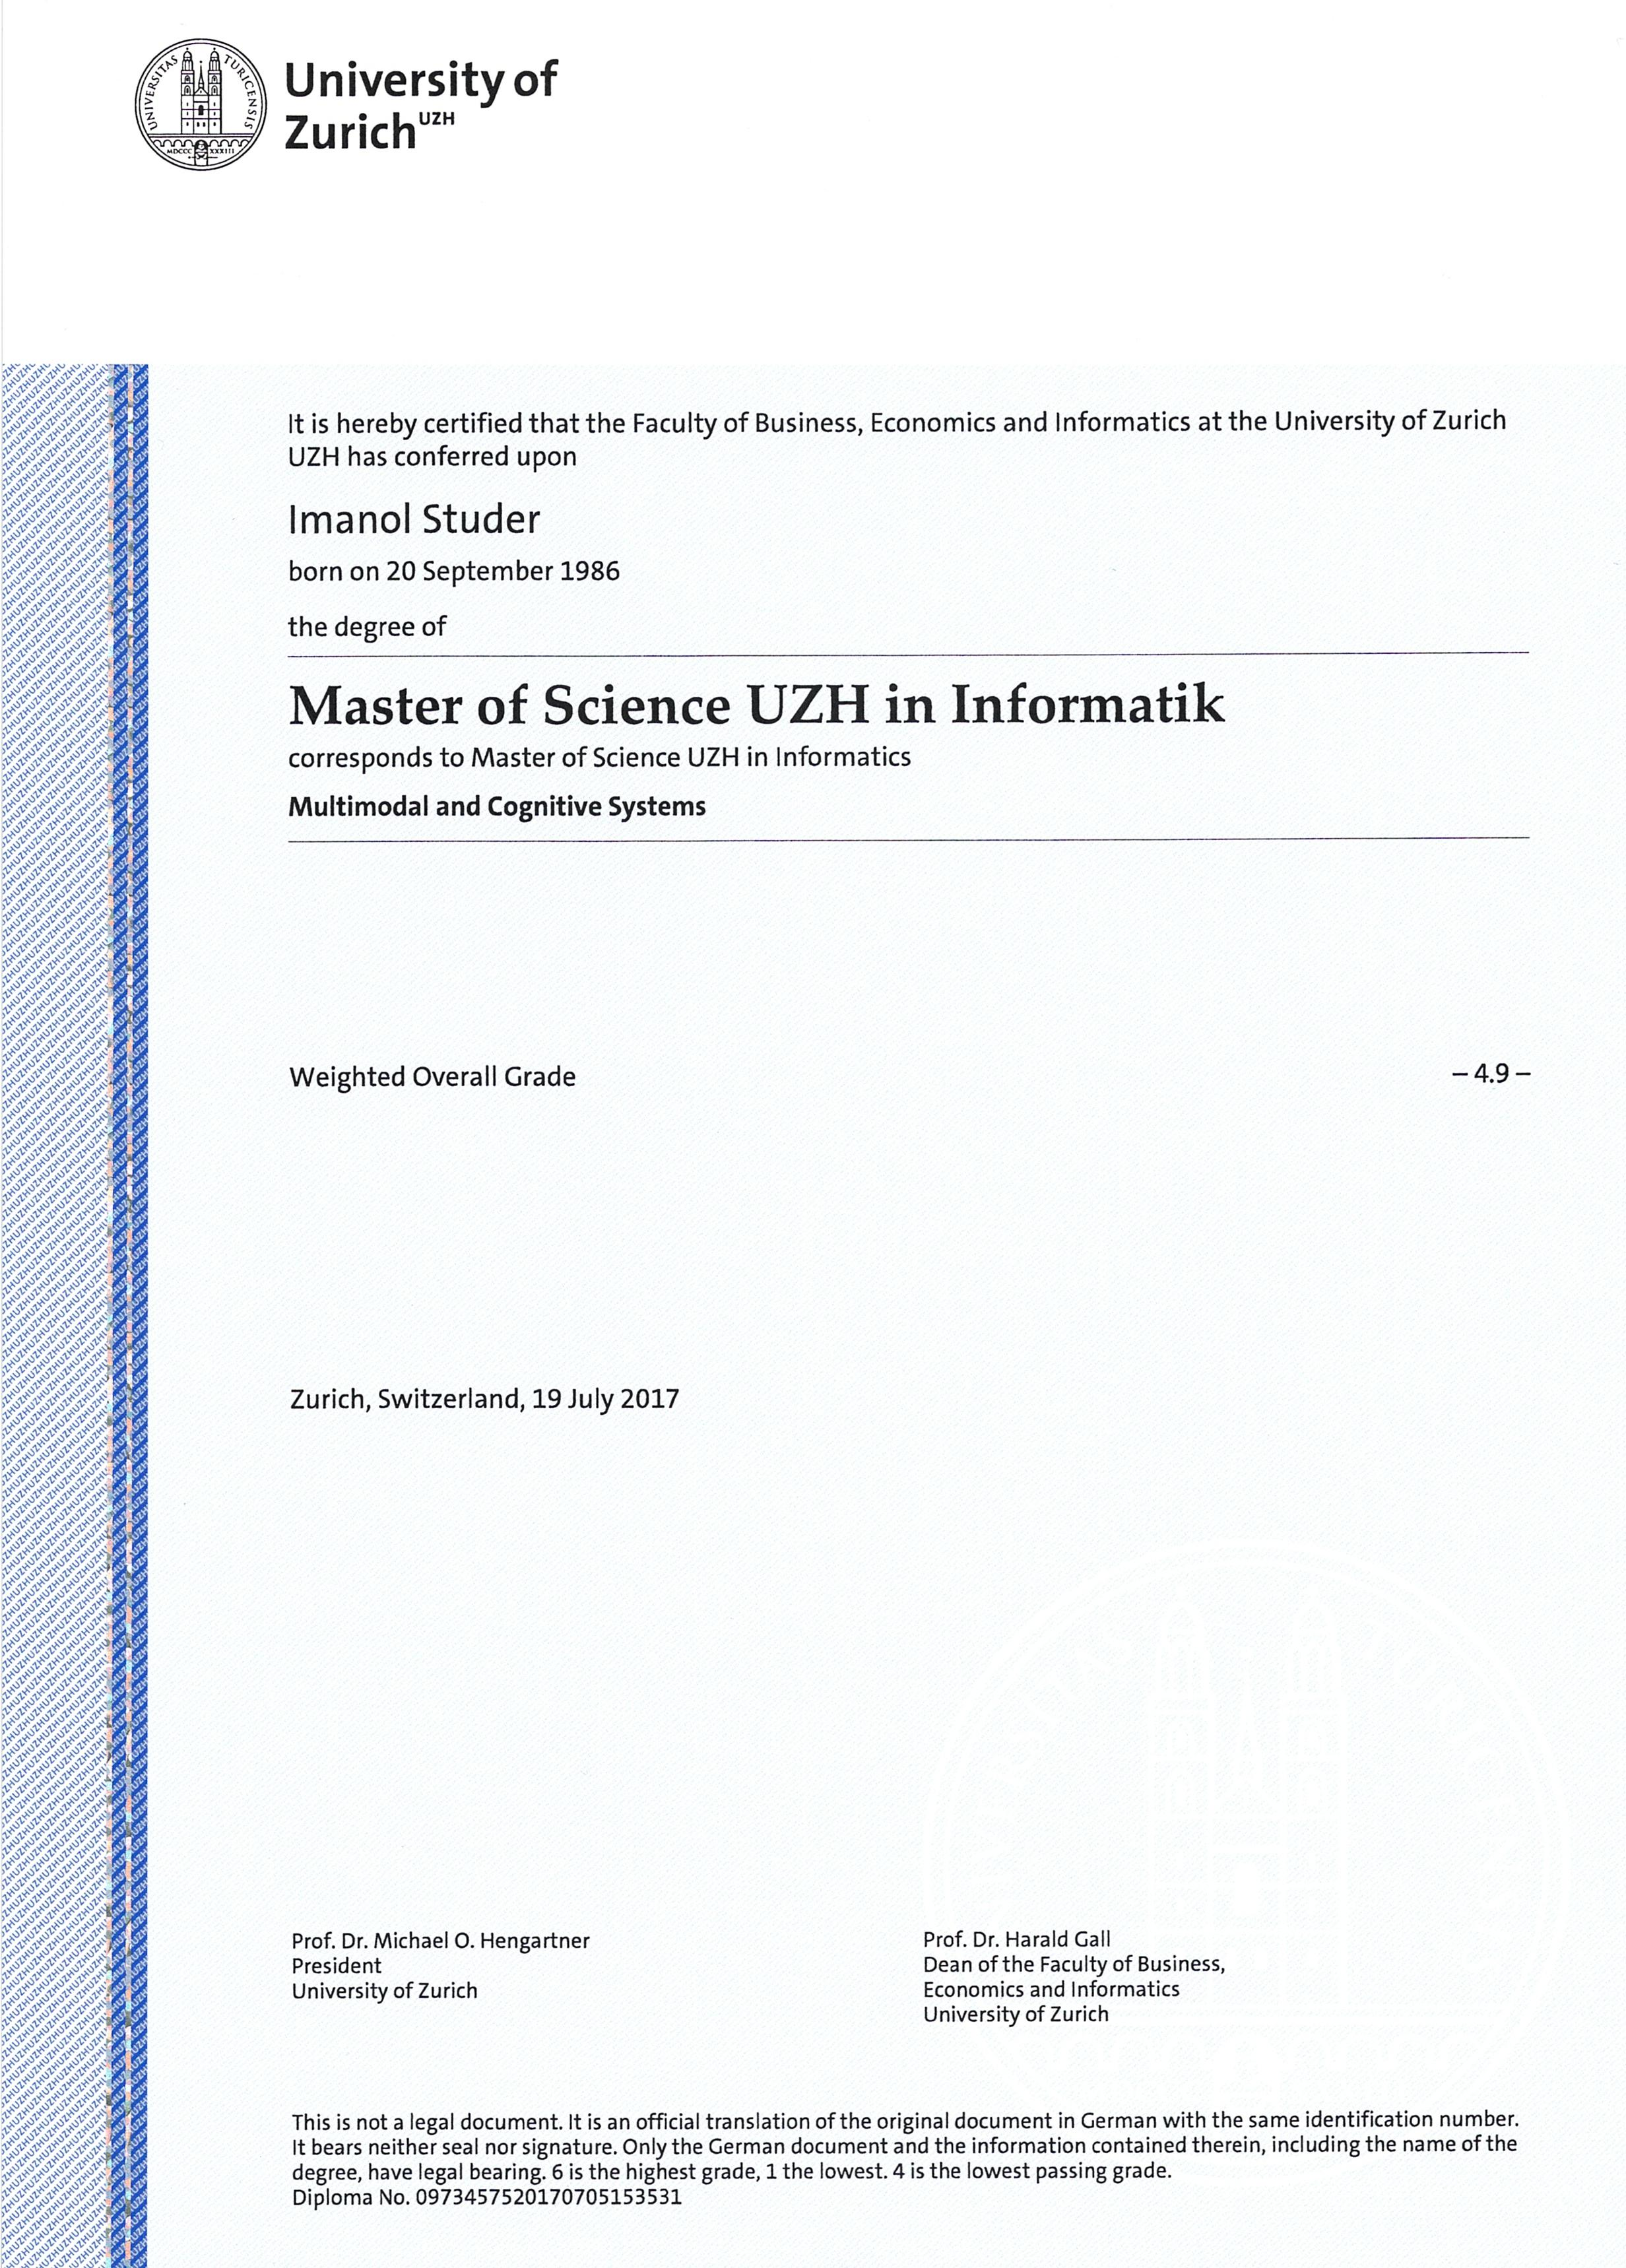
\includegraphics[width=\textwidth]{pictures/master/page0.jpg}
\newpage
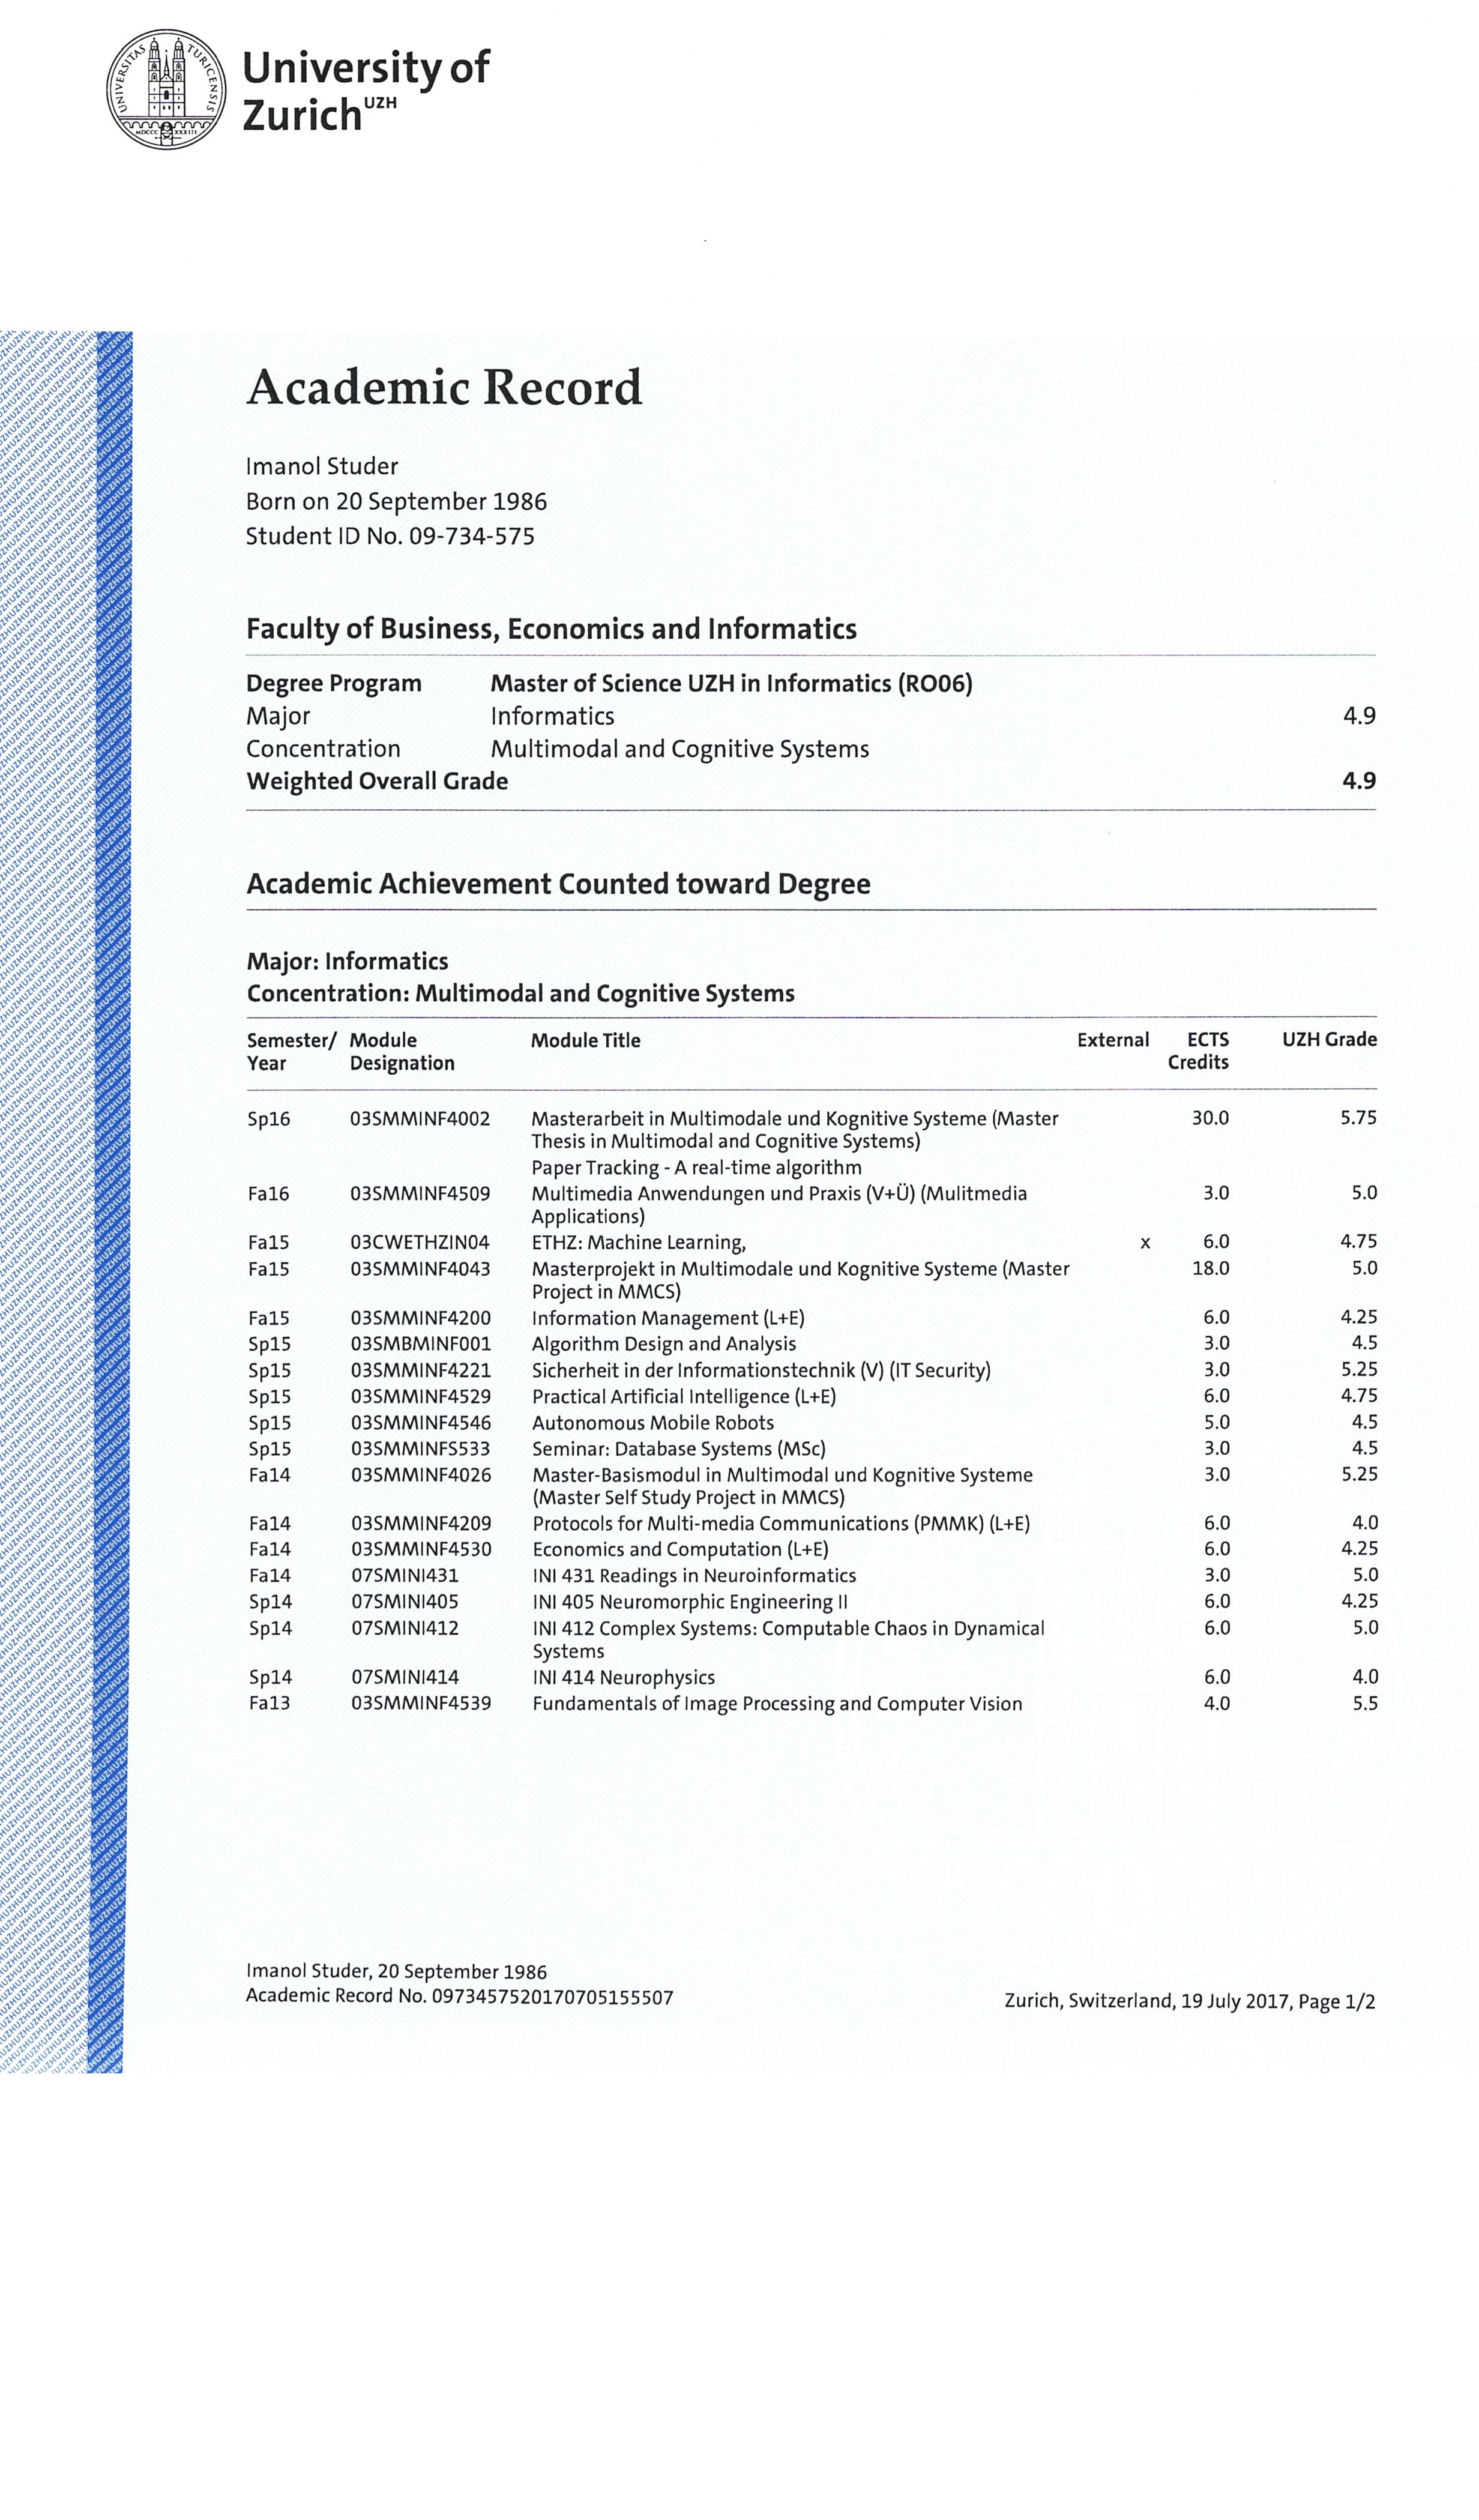
\includegraphics[width=\textwidth]{pictures/master/page1.jpg}
\newpage
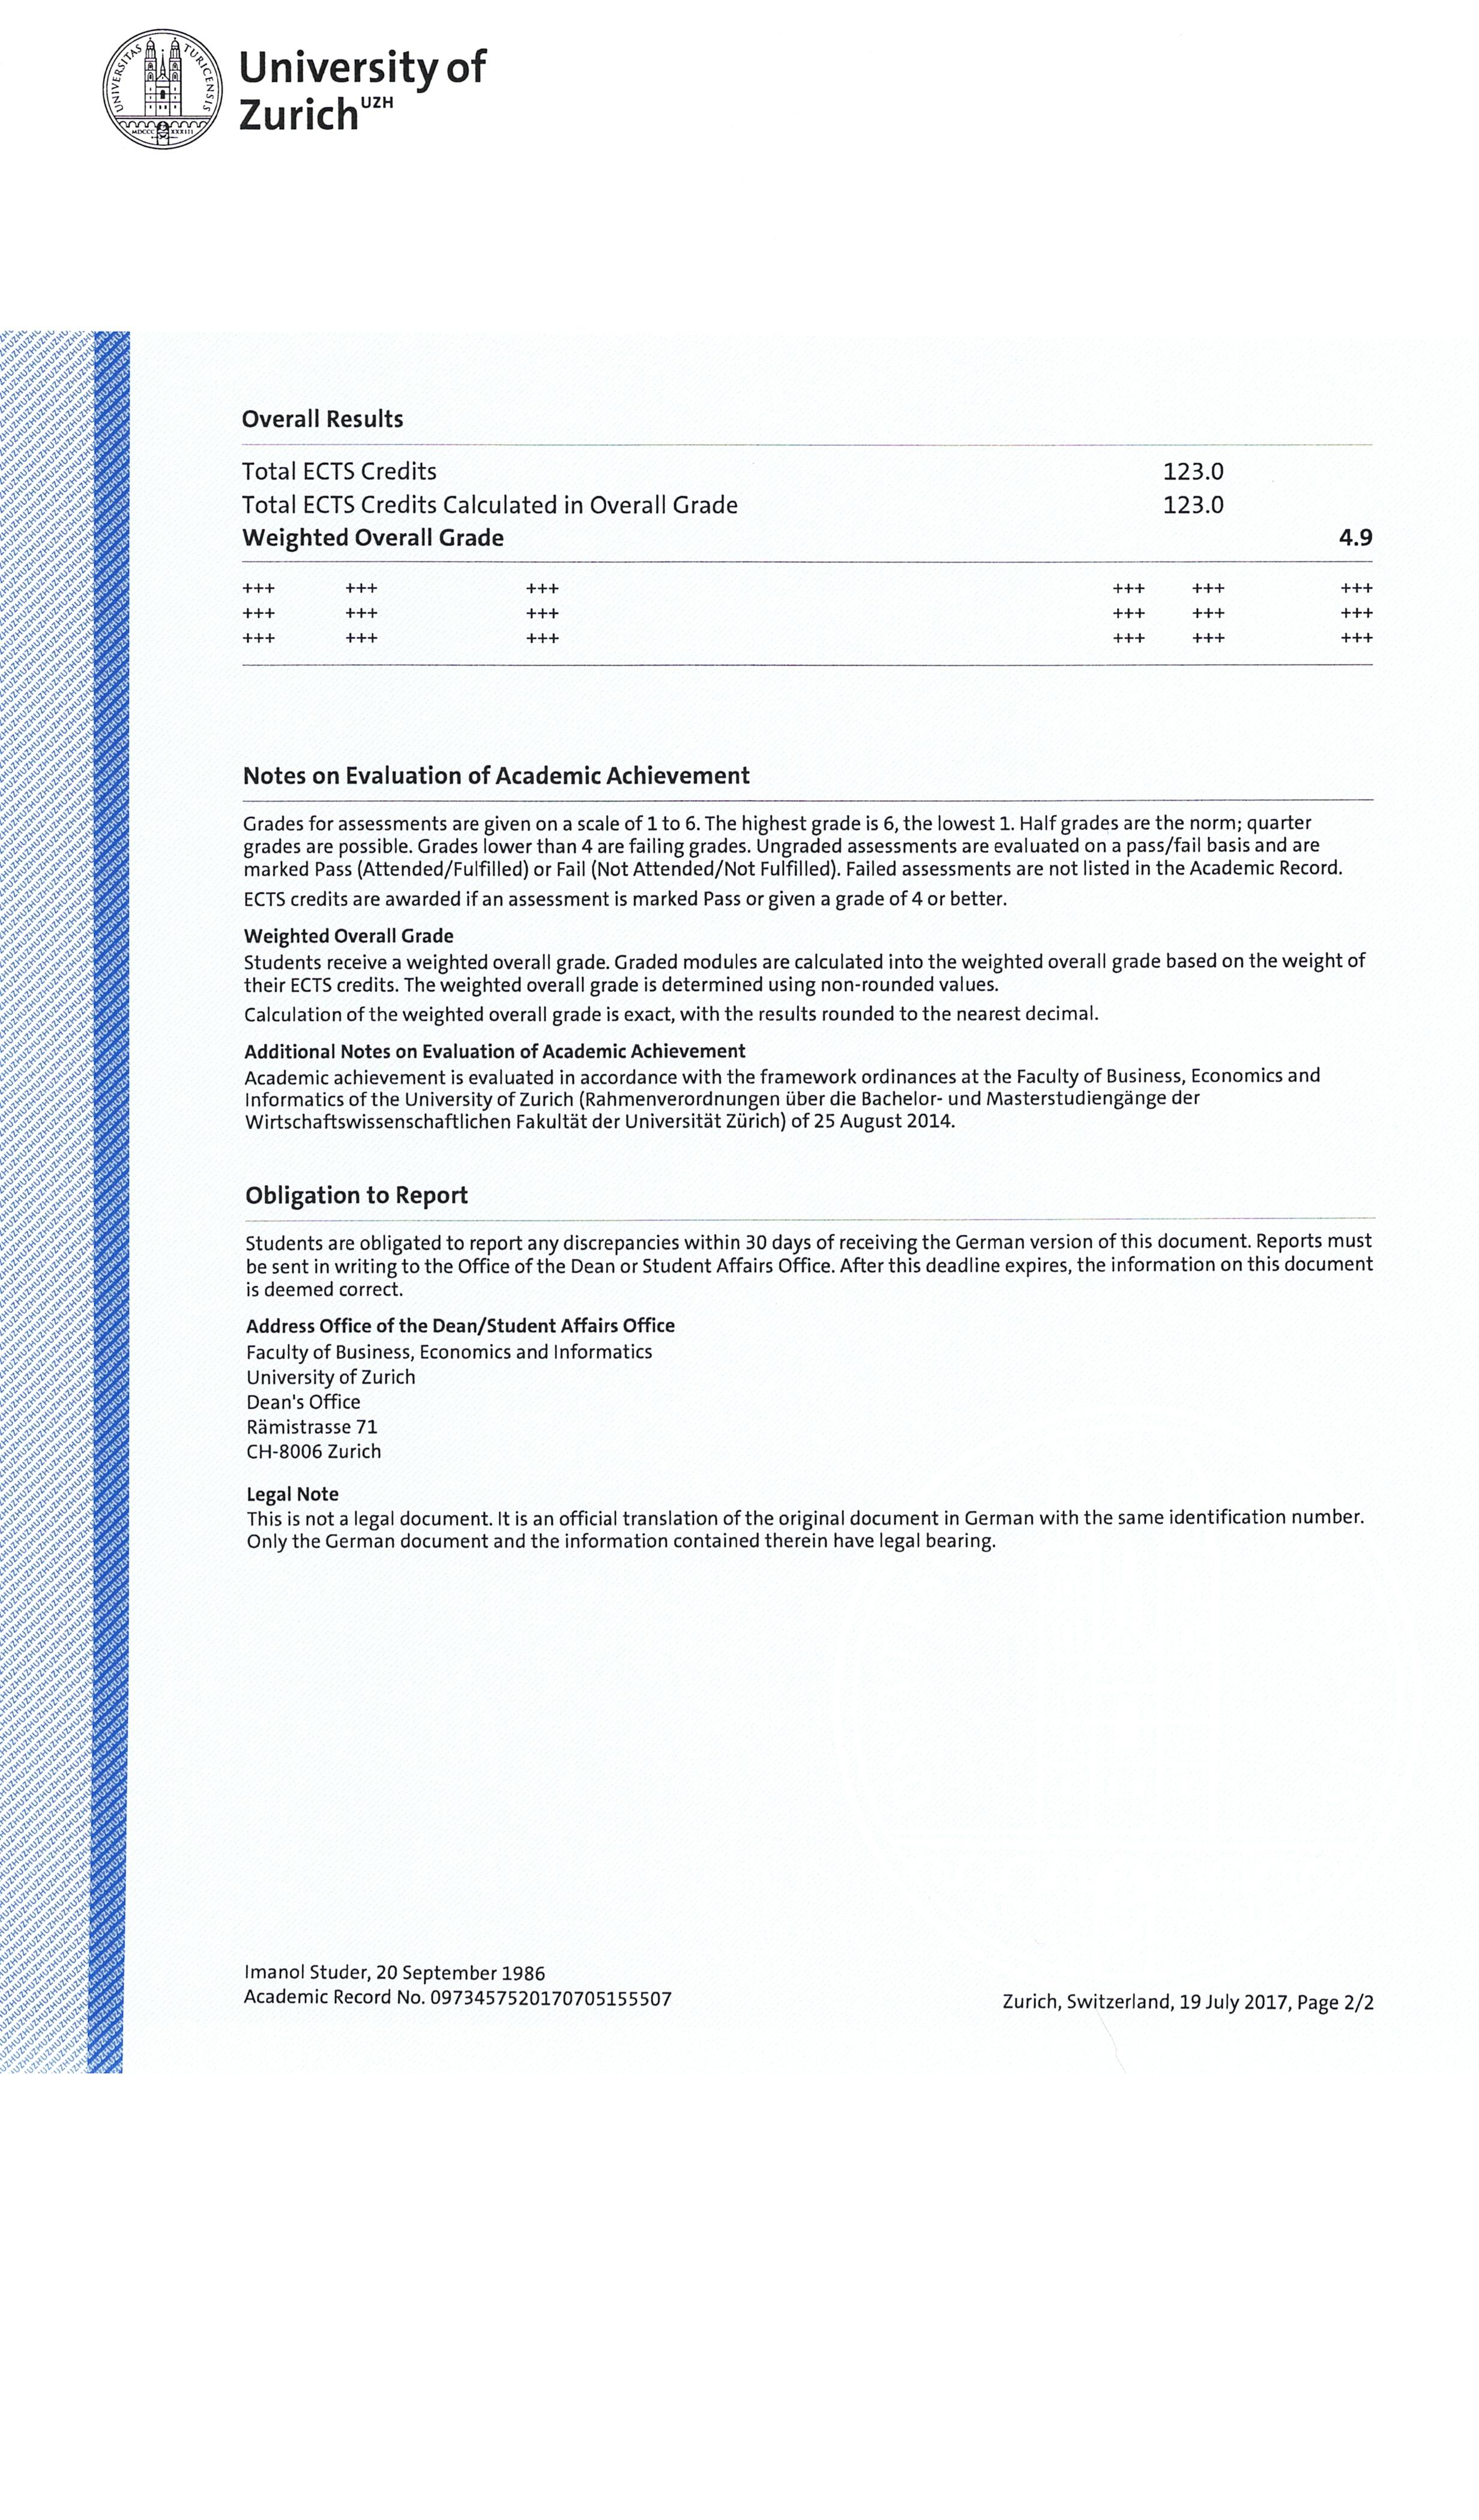
\includegraphics[width=\textwidth]{pictures/master/page2.jpg}

\enlargethispage{12pt}
\newpage
\section{Bachelor's Diploma}
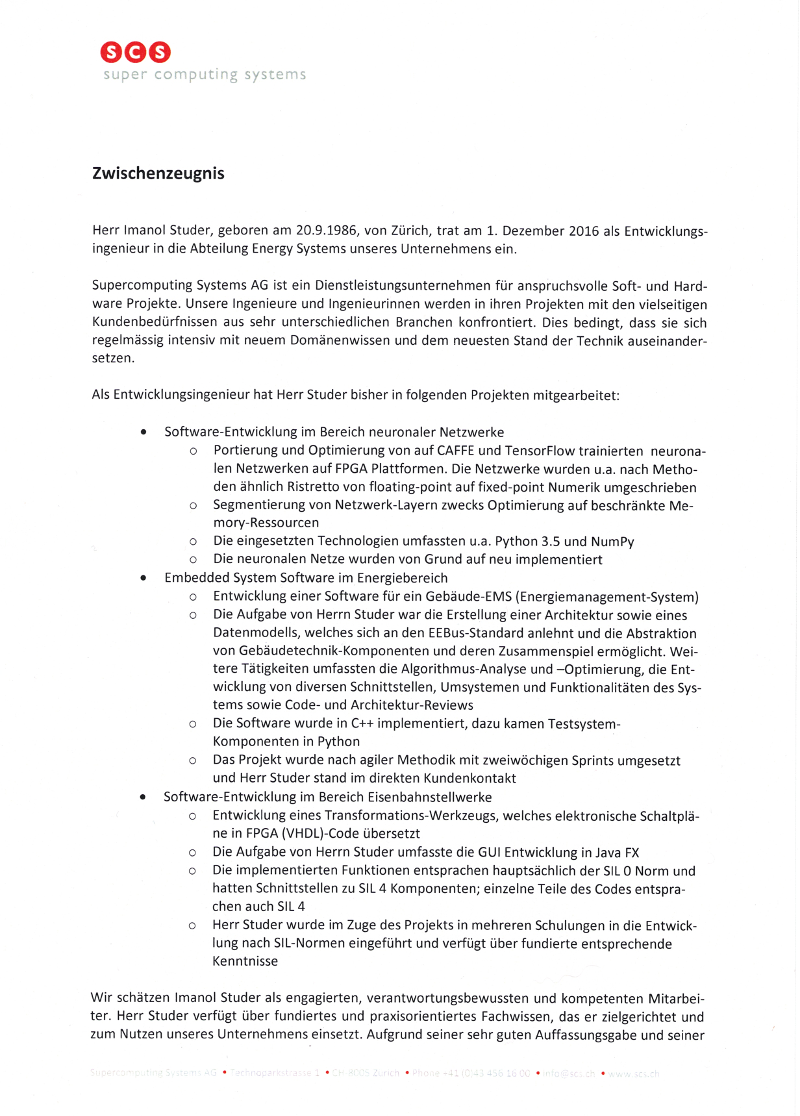
\includegraphics[width=\textwidth]{pictures/bachelor/page0.png}
\newpage
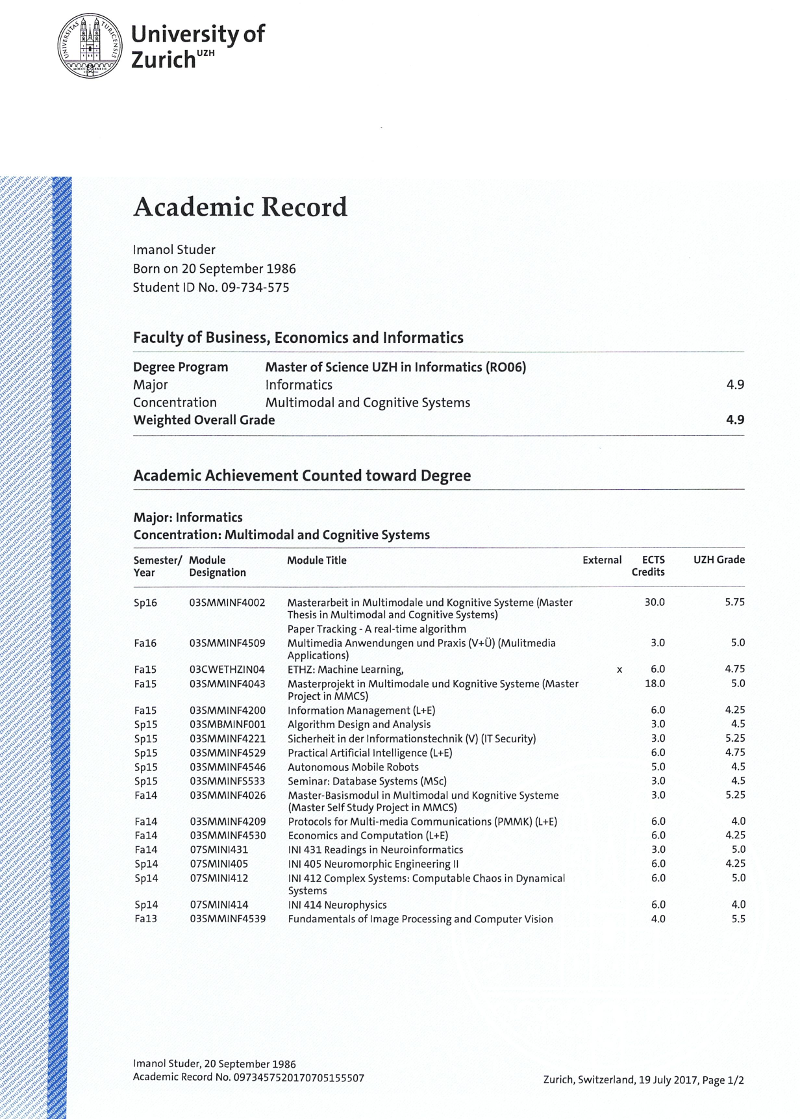
\includegraphics[width=\textwidth]{pictures/bachelor/page1.png}
\newpage
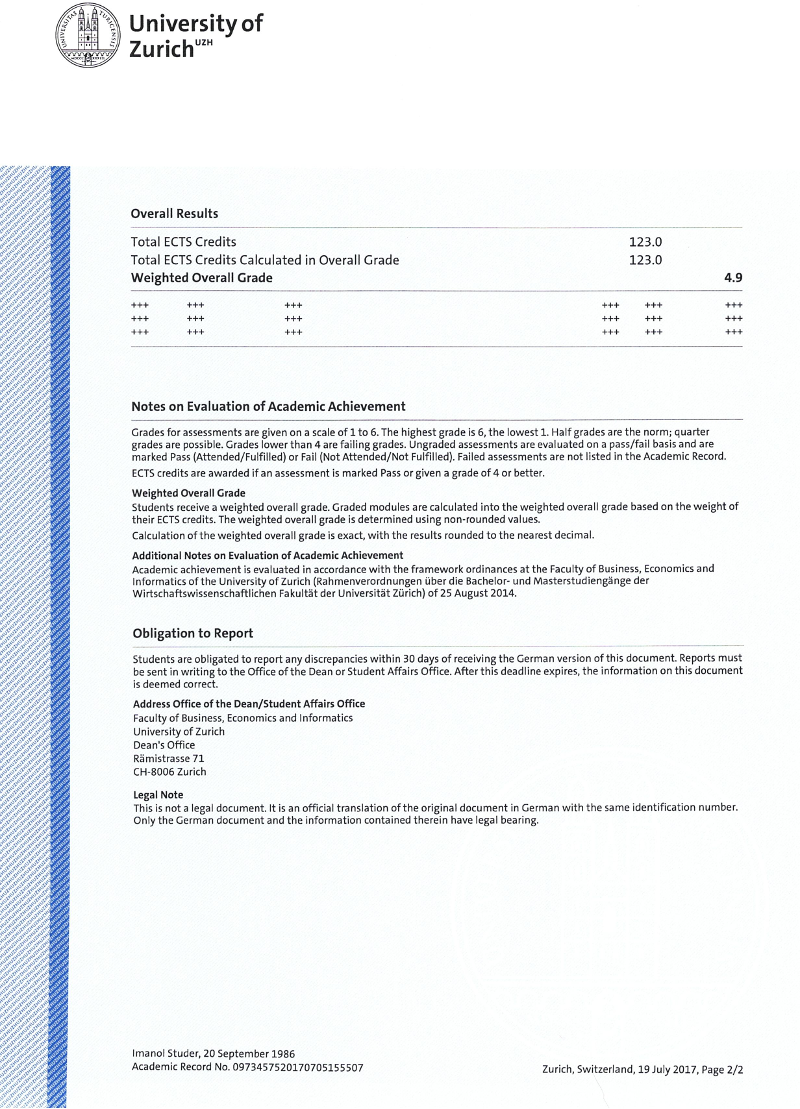
\includegraphics[width=\textwidth]{pictures/bachelor/page2.png}

\end{document}